\section{Project management}
SECTION NOT FINISHED. As mentioned earlier, the team chose scrum. Yodiz, we now wish we had chose another scrum tool. After a while we added a person responsible for some serving on our work days. Also responsible for making sure we took brakes. 
The team introduced punishments for being to late for meetings and not doing all of your assignments. This was used on a team building with some food. Did this work optimally?
\subsection{Working with the customer}
SECTION NOT FINISHED. The team tried to have meetings with the customer once a week. This worked well and the team felt that it was a good thing that the customer participated to such an extent. Write something about the problems with the customer saying he is going to do something but did not and how we solved the problems around this?

\subsection{Team organization}
SECTION NOT FINISHED.
In the beginning of the project, the team distributed roles with different responsibilities. A project leader, a deputy project leader, a scrum master, a development responsible, a test responsible and a report responsible. Almost halfway through the project it became clear that the scrum master was also the one with the most Android experience. This resulted in a lot of extra work on the scrum master, while the deputy project leader had almost no work at all. Therefore, the team reflected over the project roles and the distribution and this resulted in a change of roles. The deputy project leader became the scrum master to distribute the resources in the best possible way. After this change the teams best Android resource could focus entirely on developing and helping others. The team was very satisfied with this decision and the resource distribution worked great after the change in roles. 

Was the responsibilities of the roles good?

\subsection{Changing roles}
\label{sec:unbalancedWorkload}
During sprint five, the team evaluated whether the use of the team's available resources actually were fully exploited. It was acknowledged that our (now former) Scrum master, Per Øyvind, had the best control of the development environment, which in turn lead to that the workload he got due to his position as Scrum master and his level of expertise, was too great. The team therefore decided that Lars Erik, which previously was our deputy project leader, was the best fit to be the new Scrum master.

It was also discussed whether the position ''Project leader'' actually was necessary, as it conflicted with one of the principles in Scrum. \todo{The team decided that we in fact thought the position was necessary, as the project leader and Scrum master simply distributed the Scrum master's traditional tasks between them.} The main difference would be that the project leader would handle the administrative tasks, such as room booking for meetings and work sessions, and handle customer relations, while the Scrum master would handle the project administrative tasks, such as moderating the Scrum meetings, adding tasks to the backlog and Yodiz, and generate burn down charts.

\subsection{Choice of development methods}

The team chose to use scrum together with extreme programming. This process and why these were chosen is described in section ~\ref{sec:scrumDevProcess}. Even though Scrum is well known, many team members had different expectations to how the framework would be implemented in the project.


OMFORMULERES: Each team member spent a significant amount of time getting up to date with the Android platform and the front-end architecture of Android apps. In retrospect, more time should have been spent getting all group members up to date and practicing Android programming together in the beginning of the project. One of the team members had some experience with Android before and ended up spending a lot of time teaching and explaining to all of the other team members. If this had been organized in a way, for instance by holding a course in the beginning, some of the time spent on this could have been saved. 

\subsection{Underestimation of workload}
A prevalent risk to any project is the failure to acknowledge the cost of tasks in the project and the improper allocation of resources that follows such an error. This can also lead to a false sense of what a team can achieve in a given time frame. 

The team experienced this risk to have the biggest negative impact on our workflow. Even though it did not have much effect on the sprint end result, it was the most occurring risk, which added up to be very time consuming. The main reason for this issue was the lack of experience with many of the tasks, but also that we initially did not consider who the tasks were assigned to, which turned out to play an important role in the equation. 

\todo{explain how the team resolved this issue?}

\subsection{Choice of Scrum tool}

\subsection{Improper use of Yodiz}
\label{sec:improperScrum}
As mentioned in section~\ref{sec:scrumtool}, the team used a lot of time on
deciding on which Scrum tool to use for the project management. Although our
choice fell on Yodiz, the team was in lack of any previous experience with the
tool, and despite the team's efforts to get acquainted with the tool, a
misunderstanding arose and was not discovered until the end of the second
sprint.

The misunderstanding, displayed in figure~\ref{fig:wrongUse}, was that the team
assumed one could add multiple individuals as responsible on a particular task,
while Yodiz' functionality only assigned the time spent to the individual that
either created the task or was assigned as owner of the task.

As a result, it appeared as if only singular individuals performed the tasks,
even though the entire team in reality was participating, which was also
reflected in the burn down charts and the generated Gantt diagram. 

To sort out this issue, the team went through old meeting reports and time sheets
to figure out which members of the team that had actually participated on the
particular task, and added new tasks and the time spent to the members that at
the time had not recorded this information.%, as shown in figure~\ref{fig:addsTasks}.

This issue was unfortunate, but not insurmountable, and also not a critical
issue for the overall progress of the project.

\begin{figure}[H]
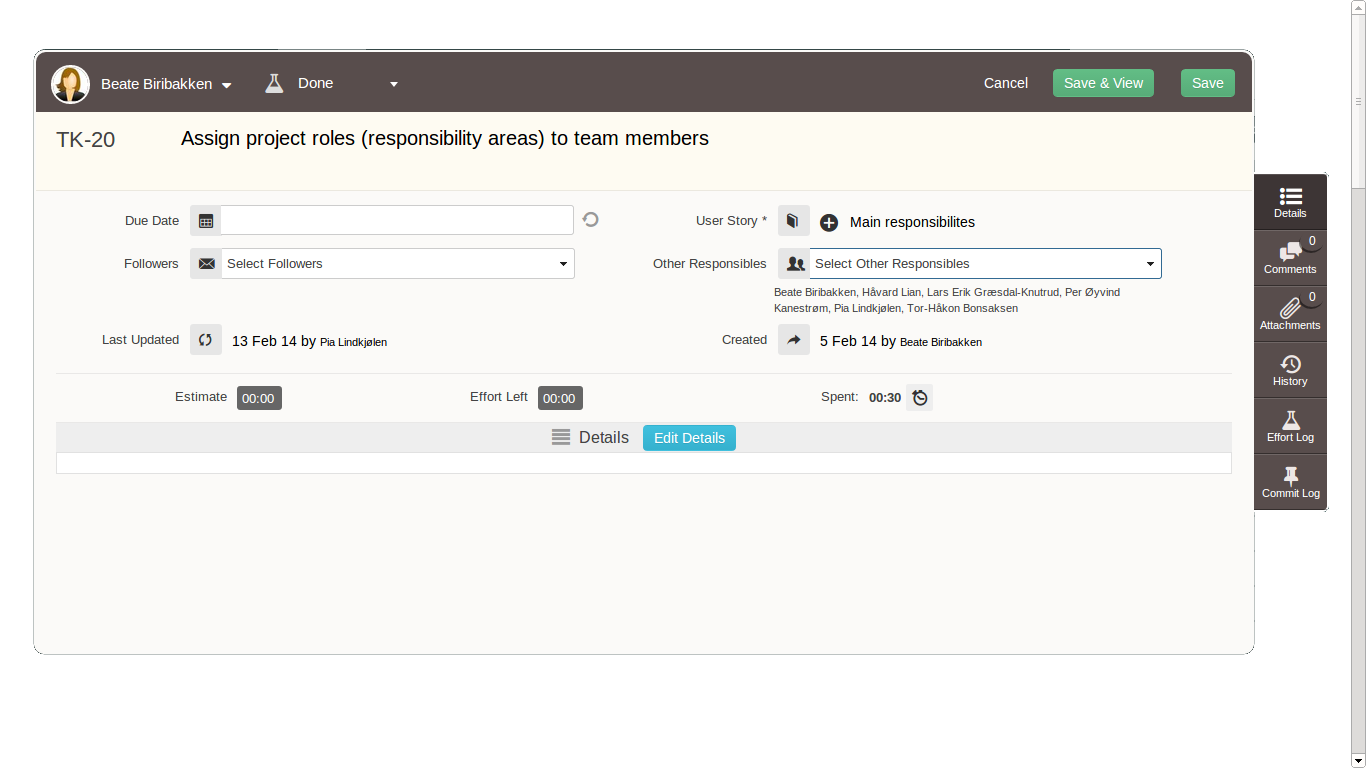
\includegraphics[width=\textwidth, clip, trim=1cm 2cm 4cm 1cm]{ch/retrospect/fig/wrongUse.png}
\caption{Example screenshot to illustrate improper use of Yodiz}
\label{fig:wrongUse}
\end{figure}